\chapter{Methodology}

\section{Problem statement}
    \subsection{Objective}
    Our primary objective is to enhance the transparency and trustworthiness of electronic elections. One way to achieve this is to provide a guarantee that election was conducted correctly, according to certain correctness criteria. We refer to the ``Software Independence" concept \cite{Rivest2008OnTN} and develop a program that issues a guarantee of correctness for an election by verifying the evidence of computations. This guarantee can be provided by a computer program known as a verifier.
    However, in order to ensure the correctness of the election, the verifier itself must be proven to be correct. This is a significant challenge due to the gap in software correctness. The solution is to employ proof-based software development, although this technology is not yet mature.

    \subsection{Scoping}
    Election verifiers are specific to a particular election because the verifiable properties differ from one election to another, as does the election protocol. The election protocol is closely dependent on the structure of the election questions, tallying method, and other factors. Therefore, it is impossible to develop a single verifier for multiple elections.
    Haines et al. \cite{Haines2019VerifiedVF} took a promising approach to this problem by demonstrating a generalized technique for developing election verifiers along with logical building blocks that are proven correct. We agree with this approach and believe that it is worth continuing and building upon their achievement.
    We follow Haines et al.'s work and improve their technique by using verified correct tools for our development, such as HOL4 Theorem Prover and CakeML compiler. These tools guarantee the correct operation of the program, which is a significant improvement over previous approaches. 

    In order to demonstrate our improvement to Haines' technique, we need to use a particular electronic election with universally verifiable properties. We kept our project close to the predecessor and used the same election properties and similar elections. Haines used a universally verifiable subset of integrity property and argued that it is the best that can be verified by an external auditor for electronic elections similar to Helios Voting. Integrity and privacy properties balance against each other, and it is impossible to verify more than those properties. Since the purpose of our work is not to verify this election, but rather to demonstrate the strategy, the availability of particular properties does not pose a problem. We strongly believe that our technique can be extrapolated and applied to other electronic elections and other election properties. For instance, building an election verifier acting from the side of an individual voter and having access to individually verifiable properties.

    The particular properties of electronic elections that we use for technique demonstration are the same as those used by our predecessor work. They are as follows:
    
    \begin{itemize}
            \item Valid ballot encryption. Before being sent to the voting platform, voters' individual choices are encrypted according to a cryptographic protocol. It is impossible for us to know what are the actual individual choices, hence we are unable to verify cast-as-intended property, however, we can verify that the encryption forms a valid ballot, with respect to the cryptographic protocol used. If this property verification fails, it might be an indication of a poison ballot attack. 
            \item Valid ballot collection. After encryption, ballots are sent to the Helios server for tallying. This property ensures that the same ballots that we witness encrypted are collected for tallying. Similar to the collected-as-cast property but without knowledge of the actual cast votes. 
            \item Valid ballot tallying. This property ensures that the ballots collected and the ballots tallied are the same ballots, as well as the published result of the election, is the result of the tally and not something else. Failure in this property might indicate that the published results are not what the voters actually collectively voted for.
    \end{itemize}

    The verification of the above properties heavily depends on the protocol settings, such as the choice of large prime numbers, and other factors. Therefore, we have to make some assumptions, which we will explain later.

    In this work, we demonstrate an improved technique developed by Haines et al. \cite{Haines2019VerifiedVF} that can be used to build an election verifier with end-to-end correct operation. We use a Helios-based election as an example to demonstrate this method and to verify the properties we have described. Our work expands on Haines et al. \cite{Haines2019VerifiedVF} by addressing the future work that was recommended in the paper.


    \subsubsection{Tools and Materials}
    In order to demonstrate our work, we have used the election from International Association for Cryptologic Research 2022 director election\footnote{https://www.iacr.org/elections/}. This election has been deployed on Helios Voting\footnote{https://vote.heliosvoting.org}.

    As we build upon the previous work \cite{Haines2019VerifiedVF}, we have used a very similar election, just from a later year. We have performed the entire development using HOL4 Theorem Prover\footnote{https://hol-theorem-prover.org}, in contrast to Coq Proof Assistant\footnote{https://coq.inria.fr}, which was used by our predecessor \cite{Haines2019VerifiedVF}. For our proofs, we have used the Abstract Algebra library in HOL4 developed by Joseph \cite{Chan2018ClassificationOF}.


    \subsubsection{Assumptions}
    The positive outcome issued by a verifier is often not enough to guarantee that an election was conducted absolutely correctly. Verifiers check some properties and often work under certain assumptions. However, it is theoretically possible to design an election with sufficient verifiable properties and develop a comprehensive election verifier that would ensure that all properties are correct.

    For the purposes of our technique demonstration, we clarify the assumptions we make:
    \begin{itemize}
    \item Public evidence data is relevant to the election under scrutiny and is not fabricated. Theoretically, some purposefully generated data may be placed under the URLs found on the election web page. The integrity property can hold for that data, but if it is bogus, the integrity of the data does not imply the integrity of the election.
    \item Public settings of the election protocol are chosen in accordance with technology guidelines. The cryptography protocol used in the election requires public settings, such as large and safe prime numbers, among others. If these settings are not selected properly, the election security and integrity can be compromised, while passing the verification.
    \item We put all the privacy out of scope because we have no opportunity to verify it, as these properties are individually verifiable. This means that we assume perfect privacy. As a side note, violations of privacy can violate elections, for example, if all the trustees for an election are malicious, they can manipulate election data by combining their private keys, and such an attack will be unnoticeable.
    \end{itemize}
            
\section{Approach}

    \subsubsection{Key Idea}
    Electronic elections operate using a Sigma Protocol, as explained in the Background section. The public evidence data which is published by the election system is, in fact, a transcript of the underlying Sigma protocol. To verify each property of the election, we check the corresponding transcript of a Sigma protocol. But how can we check if the transcript is valid? We use the Honest Verifier functionality of that Sigma protocol. Honest Verifier accepts valid transcripts by the definition of Sigma Protocol. To ensure that Honest Verifier does what it is supposed to do, we need to ensure the whole Sigma Protocol is correct. To do so, we prove the theorems about Sigma protocol stated in its definition. We then instantiate the election verifier using the same code of Sigma Protocol that was proven correct.
    
    Our development process of the verifier has two main phases: designing the Verifier and proving its correctness. These phases are not sequential, but rather interleaving, however, we will describe them sequentially. First, we describe how we build a verifier, and then we describe how the proofs work to ensure verifier correctness.

    \subsubsection{Environment}
    We rely on the HOL4 Theorem Prover for our entire development process. It offers a rich type system that is convenient for defining data types, functions, and the proving of theorems.
    We have chosen HOL over other environments because it enables us to develop both code and theorems about the correctness of that code within a single environment. Additionally, we can compile the same code with the verified compiler CakeML, which produces a proven correct operational program.
    By using this approach, we can ensure the preservation of correctness from the theoretical concept through the source code and to the operation of the compiled executable.



    \subsubsection{Verifier}
    In order to verify an election, verifier needs to accept a transcript for every corresponding property. Election properties might have different transcripts, meaning that we need a separate verifier for an election property or a combinational verifier. Such a verifier has to be able to ingest a corresponding transcript. Therefore, we need to construct a verifier whose type signature matches the transcript which it is supposed to verify. We do not define a verifier as a standalone entity, we define it within Sigma Protocol. The reason for this is that the verifier does not have a developed formal definition, and we would have to make it ourselves and prove that it suffices to ensure correctness, which is a difficult task. However, the Sigma Protocol has a formal definition, and we can ensure that it is correct simply by proving already provided theorems. Thus, the approach is to design a Sigma Protocol such that its honest verifier type signature matches the transcript we need to verify. Then we prove the correctness of the Sigma Protocol using theorems and imply that, since honest verifier is part of a correct Sigma Protocol, it must also be correct.


    \subsubsection{Public Evidence Data}
    We begin with the data, because the Election Verifier's interface is prescribed by the structure of the transcript that we need to verify. Firstly, we download the election data and examine it, taking into account the Helios election protocol specifications\footnote{https://documentation.heliosvoting.org}. Upon analyzing the data, we discovered that there are three types of transcripts in our election, each corresponding to a specific operation: ballot encryption, ballot collection, and ballot tallying. To verify these transcripts, we require three verifiers possessing the type signatures that match the transcript. We have identified the type of signatures required, therefore, we can move forward with constructing a Sigma Protocol.

    \subsubsection{Components}
    We build our work upon the findings of Haines et al. \cite{Haines2019VerifiedVF, Haines2021DidYM}. They utilised elementary components to construct an election verifier. The definitions of these components have undergone extensive scientific review in various papers \cite{Cramer1997ModularDO, Barthe2009FormalCO, Smyth2015ElectionVC}. Although we reuse their component definitions, we work in HOL4 theorem prover instead of Coq proof assistant. Therefore, we need to translate the definitions from Coq language to Standard ML. Also, we need to translate definitions from one type system (calculus of inductive constructions used by Coq) to Higher Order Logic.

    We defined the following components in our work:
    \begin{itemize}
        \item Abstract Sigma Protocol: This component provides an abstract definition of the Sigma Protocol. Specifically, it defines its functionalities in terms of abstract data types and in relation to each other.
        \item Disjunctive Combiner: Allows Prover to demonstrate knowledge of one secret that is in relation with at least one statement of two.
        \item Conjunctive Combiner: Essentially two protocols run in parallel. Allows Prover to demonstrate knowledge of two secrets that both are in relation with corresponding statement of two.
        \item Equality Combiner Allows Prover to demonstrate knowledge of one secret that is in relation to both statements of two.
        \item Schnorr Sigma Protocol
    \end{itemize}
    \newpage

    \subsubsection{Composed Sigma Protocols}
    Based on the transcript structure that we obtain from the public evidence data, we have construct the following composite Sigma Protocols using our elementary components:
    \begin{enumerate}
    \item To verify the encryption of ballots, we use the composite Sigma Protocol: 
    \textbf{Disjunction of Equality of Schnorr Sigma Protocol}
    \item To verify the encrypted vote collection, we use the composite Sigma Protocol: 
    \textbf{Equality of Schnorr Sigma Protocol}
    \item To verify the encrypted vote tallying, we use the Sigma Protocol: 
    \textbf{Schnorr Sigma Protocol}
    \end{enumerate}
    Alternatively, we could have combined all three of the above composite sigma protocol into one single protocol using Conjunctive combiner. However, the resulting protocol would be much more complex and make our work error-prone. Since Conjunctive combiner essentially runs protocols in parallel, we will work with protocols separately and combine the result later.

    \subsubsection{Election Verifiers}
    We utilise the Honest Verifier of the corresponding Sigma Protocols, that we composed above, to construct an election verifier function for each of the three properties. The Honest Verifier's type signature corresponds to the transcript, which allows for easy ingestion.

    However, there is a problem with data types. The Sigma protocol operates on algebraic types such as Abelian Groups and uses Group operations such as Group Inverse. If we were to compile such a verifier with the CakeML compiler, it would be problematic because it is a verified compiler, which means the compiled program does precisely what is written in the code. However, an algebraic group cannot be instantiated since it is not a machine type like an integer or a floating-point number. The same is true for Group operations and Group inverse. Since the compiler is precise, it will not infer that our group operation is just modulo multiplication. Thus, we have to do this ourselves.
    
    To avoid these issues, we define another new verifier that is equivalent to the previous election verifier but operates on machine types. To ensure the correctness of the new verifier, we prove a theorem in HOL that states that this new verifier is equivalent to the election verifier, under assumption that it is instantiated with prime numbers. After that, our new verifier is ready to be compiled in CakeML and used to verify the election. Also, we can trust the results, because we proved it is equivalent to the original correct verifier.
    

    \section{Proofs}
        \subsection{Overall correctness}
        We demonstrated the construction of election verifier that can be compiled with the CakeML compiler and asserted its ability to ensure election correctness. However, this is only accurate if the verifier itself is proven correct. In this section, we present a chain of high-level arguments that justify this claim in Figure 4.1. The figure's explanation can be found below it.



\begin{figure}[th!]
  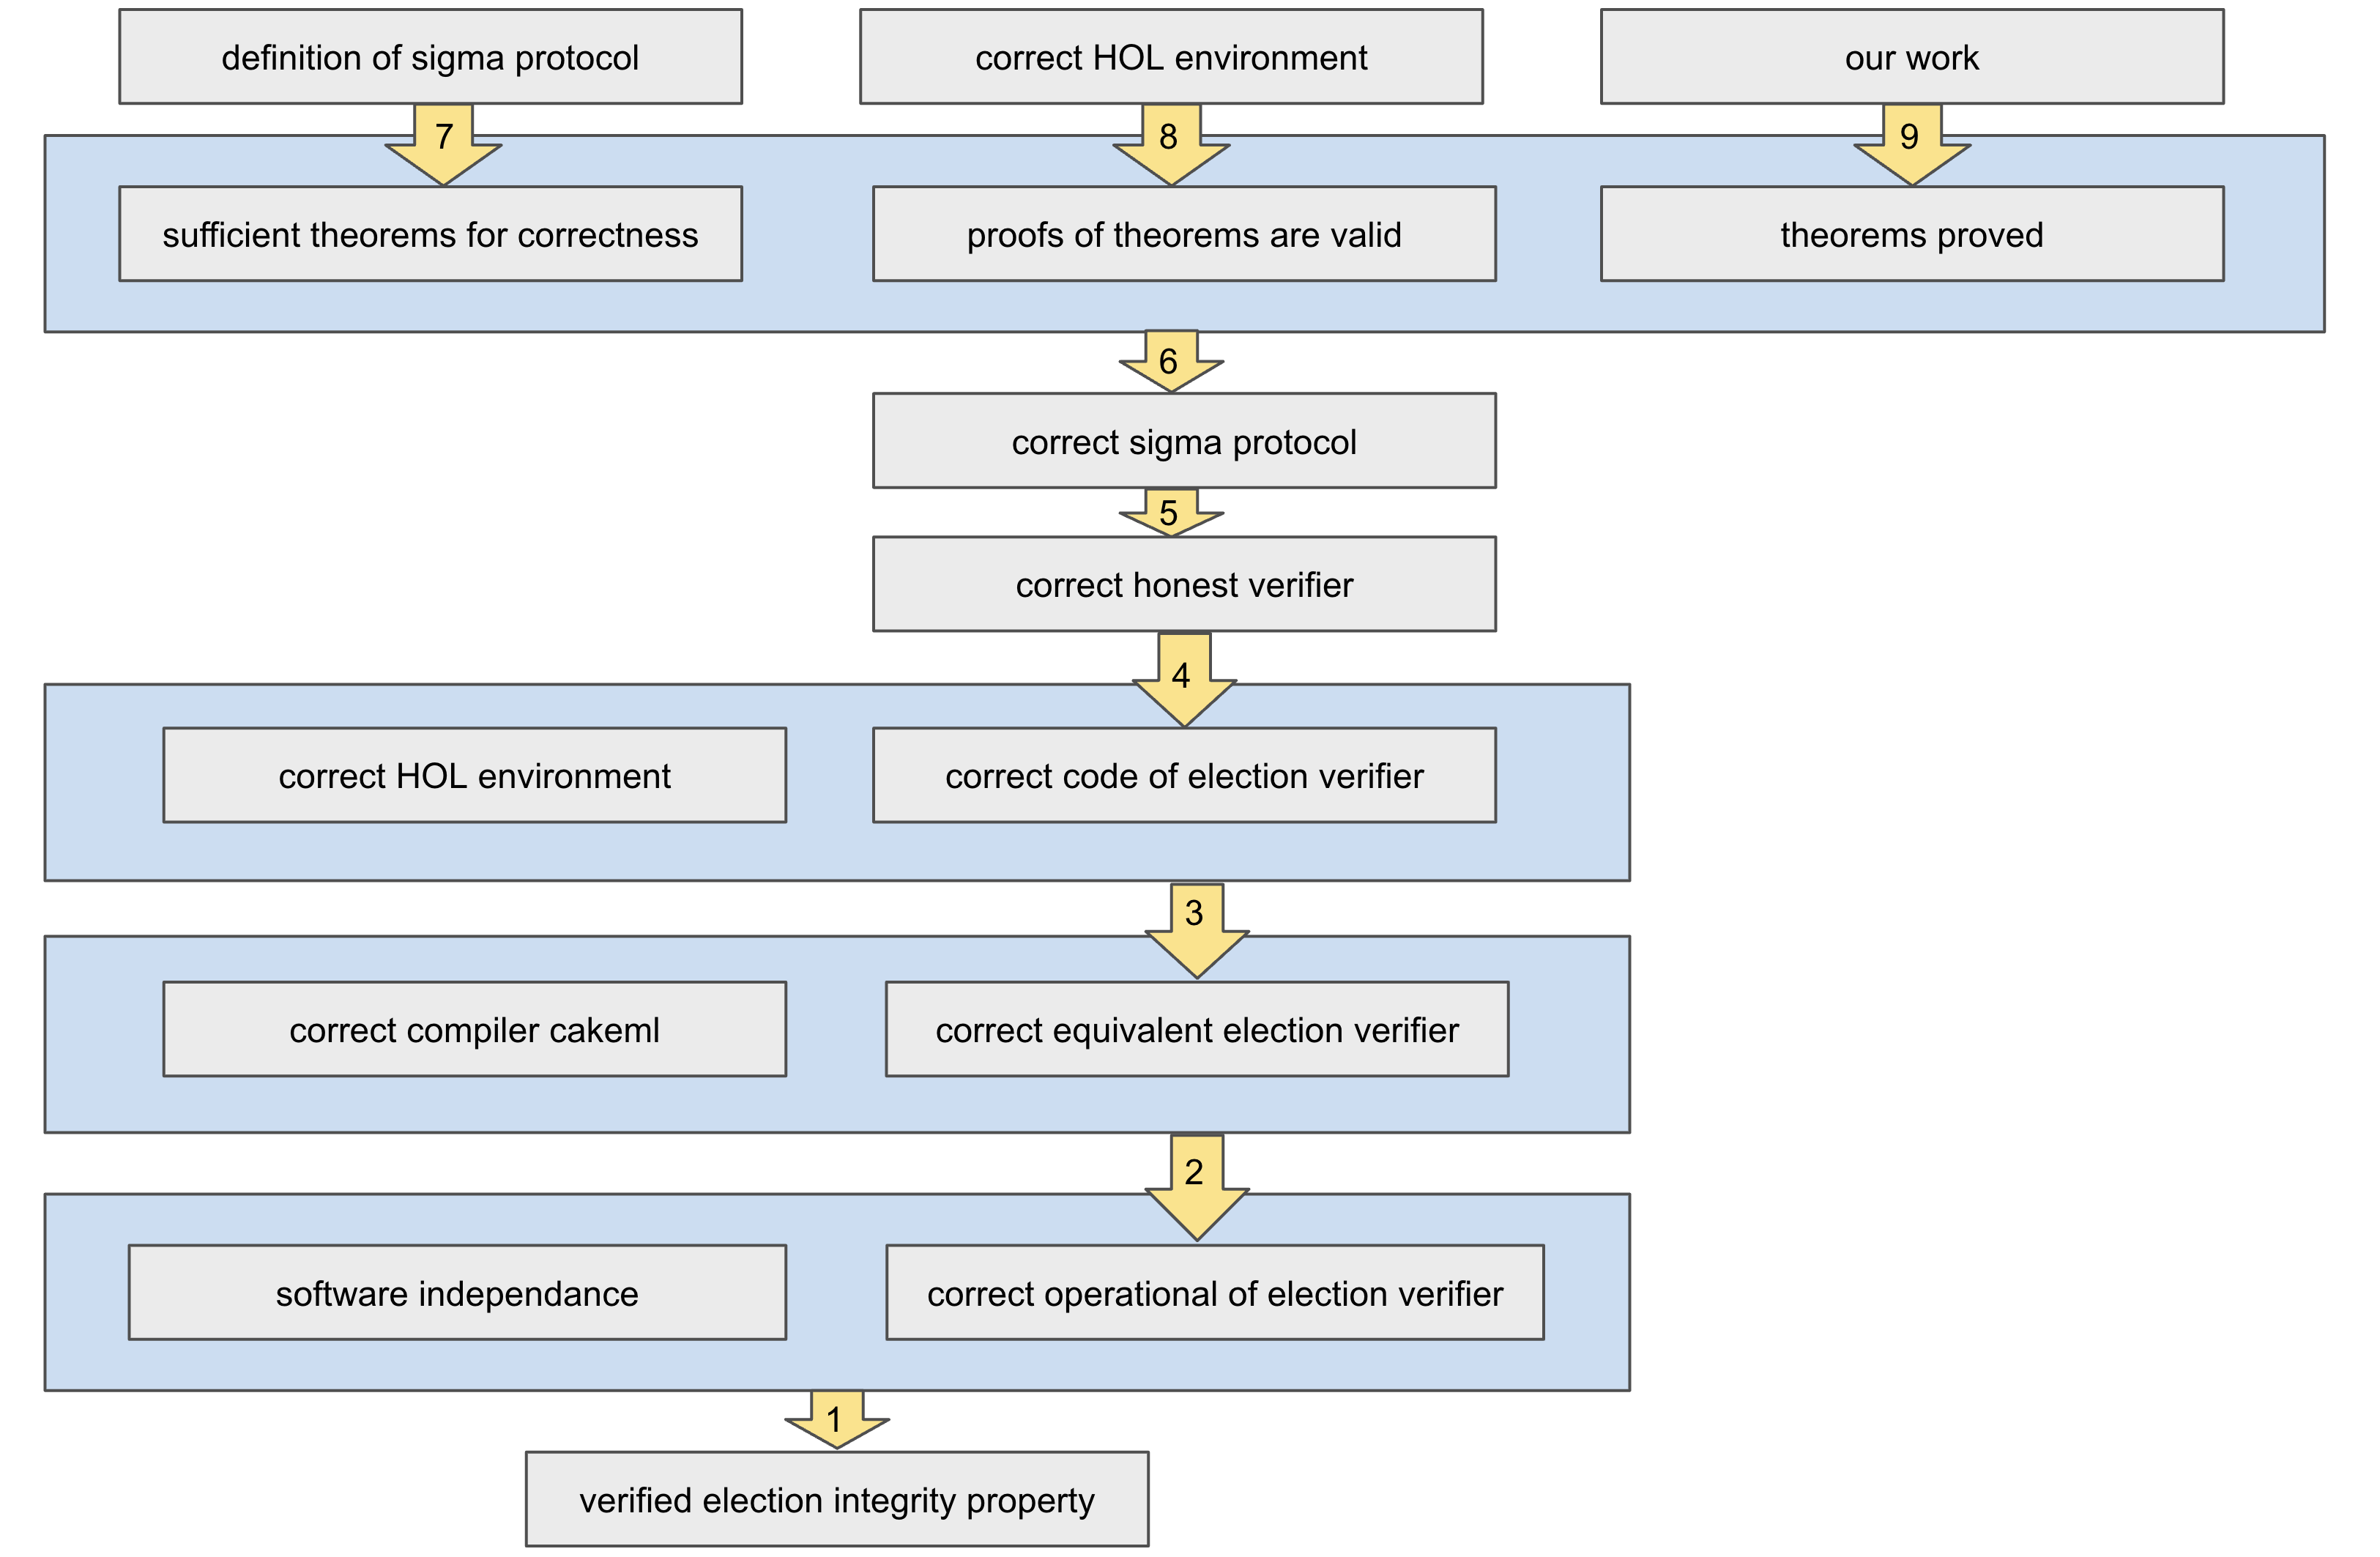
\includegraphics[width=15cm]{figures/proof_graph.png}
  \caption{Logical flow that demonstrates how the guarantee of election integrity is obtained}
\end{figure}%


    The figure demonstrates logical steps that lead to election integrity property being verified. At the bottom is the final goal, at the top is what we have to start, arrows show the implication. We trace from the goal backward and explain how every step is justified:
\begin{enumerate}
    \item Election integrity property holds because the correct election verifier accepts the transcript, supported by the ``Software Independence" concept \cite{Rivest2008OnTN}.
  \item The operational verifier program behaves correctly because the implementation of the equivalent election verifier is correct and it is compiled with verified compiler CakeML.
  \item Implementation of equivalent election verifier is correct because we prove that it is equivalent to original verifier. This proof is valid because HOL4 is verified. 
  \item The implementation of original election verifier is correct because it is calling Honest Verifier.
  \item Honest Verifier is correct because it is contained within proven correct Sigma Protocol.
  \item The Sigma Protocol is correct because
  \begin{enumerate}
      \item We proved theorems
      \item Proofs are valid
      \item Theorems are sufficient
  \end{enumerate}
  \item Theorems are sufficient because of the definition of sigma protocol \cite{damgaard2010sigma}.
  \item Proofs are valid because HOL has been proven to be able to accept only correct proofs.
  \item We proved theorems by developing the code of the proofs.
\end{enumerate}


Therefore, we have demonstrated that the verifier we constructed guarantees election correctness when compiled with the CakeML compiler. Let us now examine the important steps from the above argument in more detail.

\subsection{Sigma protocol correctness}
The correctness of the election verifier is dependent upon the correctness of the Sigma Protocol to which it belongs. In this section, we will explain how the correctness of the composed Sigma Protocol is achieved.

The correctness of the composed Sigma Protocol is dependent on the correctness of its elementary components. We utilized the Schnorr protocol and Protocol Combiners to construct the required Sigma Protocols. The correctness of the composite Sigma Protocol is a consequence of two main proven properties:
\begin{enumerate}
    \item Schnorr Sigma Protocol is correct,
    \item Correctness of the Sigma Protocol is invariant under combinations.
\end{enumerate}
In other words, we demonstrated that if the correct Sigma Protocols are combined by any of our combiners, then the resulting Sigma Protocol is also correct. Therefore, the Schnorr Protocol combined by the Equality (or any other) combiner is correct. Additionally, the Disjoint combination of the Equality Combination of the Schnorr protocol also preserves correctness.

The proofs are valid because the HOL environment guarantees that false proofs cannot be accepted. 
Moreover, the correctness property is given by the thorems which are the definition of the Sigma Protocol, so they suffice for Sigma Protocol Correctness. 
to. We believe that this strategy is sound and that it will allow us to prove the correctness of the election verifier.

We will now provide further details on how we prove the correctness of the Sigma Protocol using its definition. In order to correctly formulate our theorems, we need to clarify certain details. Since Helios uses a Zero Knowledge Proof of Knowledge, we need our Sigma Protocol to satisfy the Zero Knowledge Proof of Knowledge Definition \cite{damgaard2010sigma} discussed in the Background chapter. Namely, the three properties of Completeness, Soundness, and Zero-Knowledge must be satisfied.

\begin{itemize}
\item \textbf{Completeness:} This property can be directly defined by translating English language to mathematics or adopted from Haines et. al. \cite{Haines2019VerifiedVF}. This property states that if the Prover's statement is true, the Verifier always accepts.

\item \textbf{Soundness:} This property is defined probabilistically, which can be challenging to prove using a Proof Assistant. Thankfully, it was shown by Damgard et al. \cite{damgaard2010sigma}, that there is a stronger property Special Soundness, that does not involve probability and implies Soundness. Haines et al. \cite{Haines2021DidYM} adopted the definition of Special Soundness precisely from Damgard et al. \cite{damgaard2010sigma} and formulated in Coq theorem prover, and we will adopt it from Haines. Thus, by proving Special Soundness with this definition, we achieve Soundness. Specifically, this property states:

``For any statement $x$ and any pair of accepting conversations on $x$, $(a,e,z)$, $(a,e',z')$ where $e \neq e'$, one can efficiently compute $w$ such that $(x, w) \in R$"\cite{Haines2021DidYM}.

\item \textbf{Honest-verifier Zero-knowledge:} Honest-Verifier Zero-Knowledge is also defined using probability by Damgard \cite{damgaard2010sigma} as follows 

    ``There exists a polynomial-time simulator M, which on input x and a random e outputs an accepting conversation of the form (a, e, z), with the same probability distribution as conversations between the honest P, V on input x" 
    
    Haines in \cite{Haines2021DidYM} updated the formulation of this property, arguing that it ``suffices to show a bijection between the set of randomness and set of responses such that the output of the respective functions are equal".  We adopt the definition of Honest-verifier zero-knowledge from \cite{Haines2021DidYM} precisely.
\end{itemize}
    By proving the above three theorems we can verify that Sigma protocol is correct by definition.

\section{Summary}
We have developed an election verifier that is proven correct and able to be compiled to verify election integrity. We used Honest Verifier from Sigma Protocol, which is equivalent to the Sigma Protocol of the Election under consideration. To achieve this, we constructed a Sigma Protocol whose Honest Verifier's type signature matched the transcript that needed to be verified. We used elementary components to construct this matching Sigma Protocol.

To prove the correctness of our election verifier, we demonstrated that the Sigma Protocol that contains an equivalent verifier satisfies its definition. This proof relies on the correctness of the components and the invariance of correctness properties under the combinations of Sigma Protocols. We reused the definitions of components and formulations of theorems from \cite{Haines2019VerifiedVF, Haines2021DidYM}.

Our entire development process took place in HOL environment, ensuring that the proofs of our theorems are valid. Additionally, we developed an implementation of the verifier that can be compiled with the CakeML compiler, preserving correctness and producing a proven correct operational election verifier.




